\documentclass{article}

\usepackage{graphicx}
\usepackage{tikz}
\usepackage{tikzsymbols}
\usetikzlibrary{calc,patterns,shapes.geometric}
\pagestyle{empty}
\usepackage[margin=0pt]{geometry}
\geometry{papersize={14in,12in}}

\def\centerarc[#1](#2)(#3:#4:#5){\draw[#1] ($(#2)+({#5*cos(#3)},{#5*sin(#3)})$) arc (#3:#4:#5);}

\begin{document}
	\begin{figure}
		\centering
		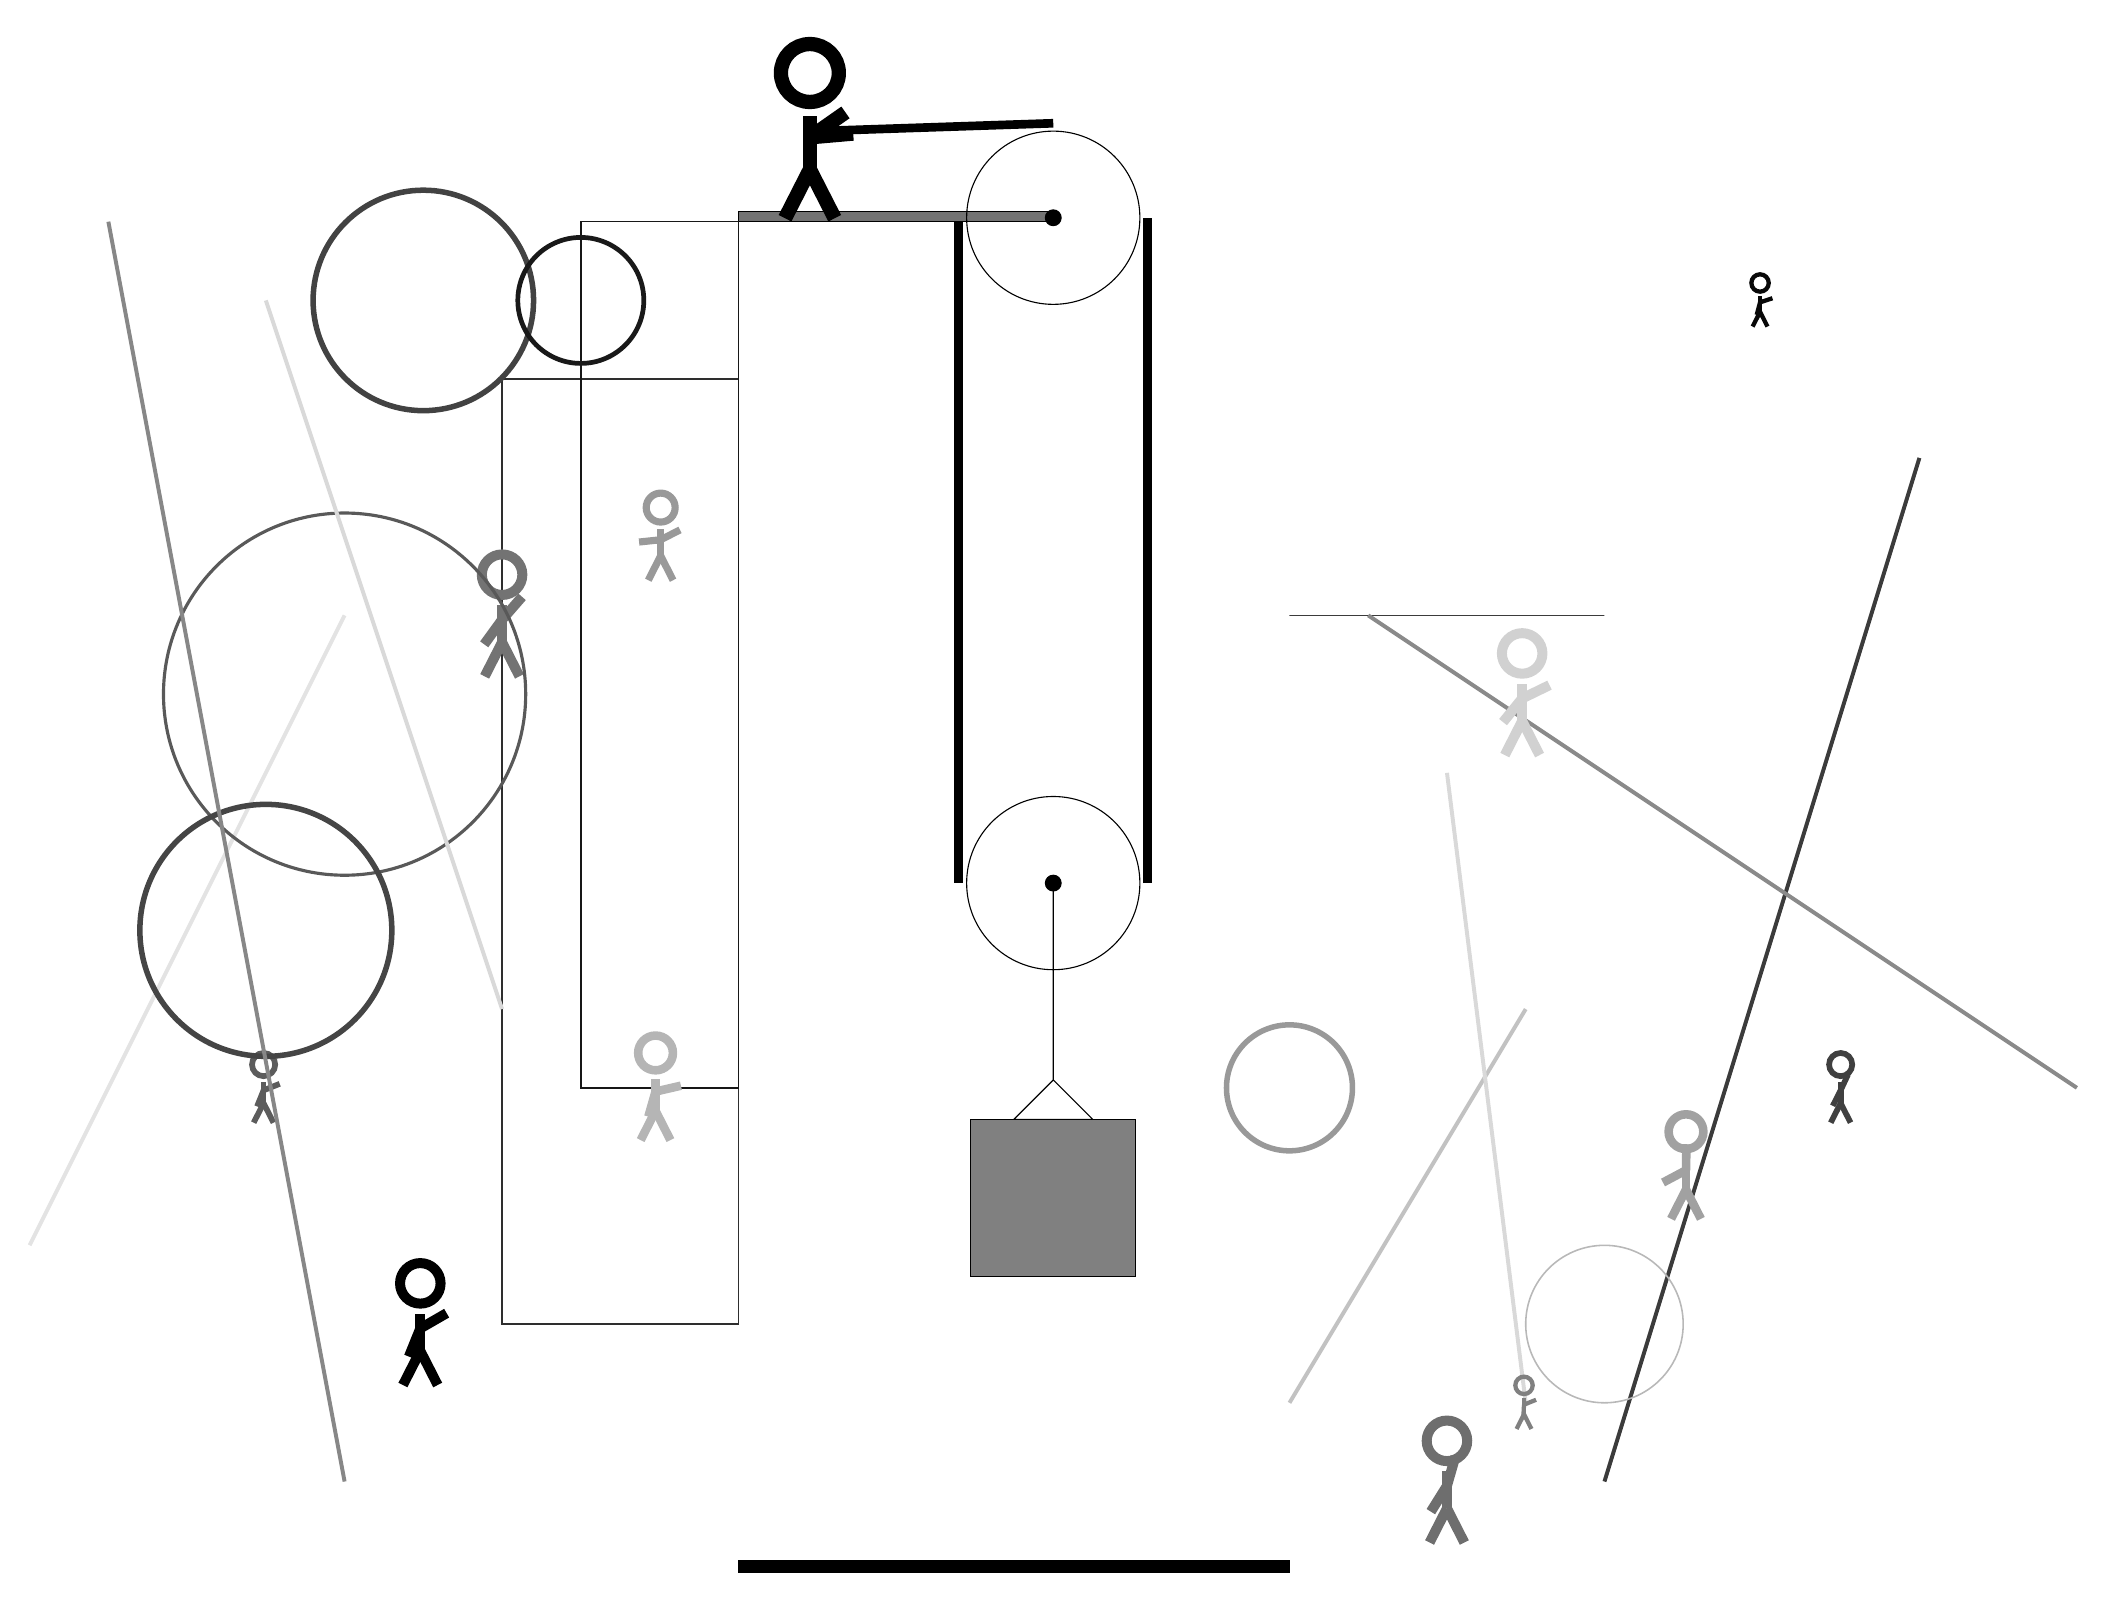
\begin{tikzpicture}
			%%%%% START %%%%%
			
			\draw[fill=black!55] (-2, 14) rectangle (2, 14.125);
			
			\draw (2, 5.6) circle (1.1);
			\draw[fill=black] (2, 5.6) circle (0.1);
			
			\draw (2, 14.05) circle (1.1);
			\draw[fill=black] (2, 14.05) circle (0.1);
			
			\draw (2, 5.6) -- (2, 3.1) -- (1.5, 2.6) -- (2.5, 2.6) -- (2, 3.1);
			\draw[fill=black!50] (0.95, 2.6) rectangle (3.05, 0.6);
			
			\draw[line width=1.1mm] (0.8, 14) -- (0.8, 5.6);
			\centerarc[line width=1.1mm](2, 5.6)(180:360:1.2000000000000002);
			\draw[line width=1.1mm](3.2, 5.6) -- (3.2, 14.05);
			\centerarc[line width=1.1mm](2, 14.05)(0:90:1.2000000000000002);
			\draw[line width=1.1mm](2, 15.25) -- (-1, 15.15);
			
			\node at (-1, 15.15) {\Strichmaxerl[10][-175][35]};
			
			\draw[line width=0.2mm, color=black!82] (-2, 0) rectangle (-5, 12);
			
			\node[line width=0.7mm, color=black!55] at (-5, 9) {\Strichmaxerl[7][54][49]};
			\draw[line width=0.2mm, color=black!91] (-4, 14) rectangle (-2, 3);
			\draw[line width=0.5mm, color=black!24](5, -1) -- (8, 4);
			\draw [line width=0.7mm, color=black!40](5, 3) circle (0.8);
			\node[line width=0.6mm, color=black!29] at (-3, 3) {\Strichmaxerl[6][74][13]};
			
			\draw[line width=0.5mm, color=black!77](9, -2) -- (13, 11);
			
			\node[line width=0.2mm, color=black!40] at (-3, 10) {\Strichmaxerl[5][6][27]};
			\node[line width=0.5mm, color=black!100] at (-6, 0) {\Strichmaxerl[7][68][30]};
			\draw[line width=0.5mm, color=black!11](-7, 9) -- (-11, 1);
			\node[line width=0.4mm, color=black!37] at (10, 2) {\Strichmaxerl[6][28][89]};
			\draw[line width=0.2mm, color=black!77] (5, 9) rectangle (9, 9);
			\draw [line width=0.2mm, color=black!28](9, 0) circle (1.0);
			
			\draw[line width=0.5mm, color=black!15](7, 7) -- (8, -1);
			\draw[line width=0.5mm, color=black!46](6, 9) -- (15, 3);
			\node[line width=0.7mm, color=black!64] at (-8, 3) {\Strichmaxerl[4][68][22]};
			
			\node[line width=0.4mm, color=black!75] at (12, 3) {\Strichmaxerl[4][63][65]};
			
			\node[line width=0.6mm, color=black!97] at (11, 13) {\Strichmaxerl[3][75][18]};
			\draw [line width=0.6mm, color=black!88](5, 9) circle (0.0);
			
			\draw [line width=0.7mm, color=black!74](-6, 13) circle (1.4);
			\draw [line width=0.4mm, color=black!65](-7, 8) circle (2.3);
			
			\draw [line width=0.7mm, color=black!73](-8, 5) circle (1.6);
			\draw [line width=0.6mm, color=black!90](-4, 13) circle (0.8);
			\node[line width=0.4mm, color=black!57] at (7, -2) {\Strichmaxerl[7][58][74]};
			\draw[line width=0.5mm, color=black!15](-5, 4) -- (-8, 13);
			\node[line width=0.5mm, color=black!50] at (8, -1) {\Strichmaxerl[3][87][22]};
			\draw[line width=0.5mm, color=black!47](-7, -2) -- (-10, 14);
			\node[line width=0.7mm, color=black!18] at (8, 8) {\Strichmaxerl[7][51][26]};
			
			\draw[fill=black] (-2, -3) rectangle (5, -3.15);
			
			%%%%% END %%%%%
		\end{tikzpicture}
	\end{figure}	
\end{document}